% Chinese backup of ../main.tex: same content, numbers and figures. Build with XeLaTeX:
%   cd report/zh && latexmk -xelatex main.tex
% Keep it in step with the English sources whenever those change.
\documentclass[conference]{IEEEtran}
\usepackage[UTF8,scheme=plain,fontset=mac]{ctex}
\usepackage{amsmath,amssymb}
\usepackage{booktabs}
\usepackage{graphicx}
\usepackage{url}
\usepackage[hidelinks]{hyperref}
\usepackage{xcolor}
\usepackage{algorithm}
\usepackage{algpseudocode}
\setmainfont{Times New Roman}
\setsansfont{Arial}
\setmonofont{Courier New}
\graphicspath{{../}}
\renewcommand{\abstractname}{摘要}
\renewcommand{\refname}{参考文献}
\renewcommand{\tablename}{表}
\renewcommand{\figurename}{图}
\renewcommand{\IEEEkeywordsname}{关键词}
\floatname{algorithm}{算法}
\algrenewcommand\algorithmicrequire{\textbf{输入：}}
\algrenewcommand\algorithmicfor{\textbf{对}}
\algrenewcommand\algorithmicdo{\textbf{执行}}
\algrenewcommand\algorithmicend{\textbf{结束}}
\linespread{1.08}
% Mark text still to be written; none may remain at submission.
\newcommand{\todo}[1]{\textcolor{red}{[#1]}}

\title{基于实测加性的分块下降：\\二十次调用下的批量黑箱调参}

\author{\IEEEauthorblockN{张子木、刘润泽、艾子齐、胡馨澜、武韵扬}
\IEEEauthorblockA{SDM374 机器学习系统设计，南方科技大学}}

\begin{document}
\maketitle

\begin{abstract}
我们调节三栋建筑能源控制器的 21 个目标权重，以最小化区域净负荷的爬坡量 $R$；$R$ 由一个确定性仿真器测得，预算为 20 次
顺序调用、每次 50 个点，且首次调用前只能使用 2,048 行训练数据。远离数据处的代理模型最优解偏乐观 8--43~kWh，因此我们让实测
而不是预测来驱动搜索。在\emph{加性分块下降}中，每个候选只改动一栋建筑，使每个点都成为效果可归因的实验；下一次调用把各
建筑的改进组合起来，组合的值仅凭这些实测效果来预测。在真实仿真器上的完整预演中，组合贡献了 33\,\% 的下降，其加性预测误差
为 0.17~kWh，而代理模型挑选点的误差为 4.9。去掉分块结构、其余不变，平均最终 $R$ 在六个种子上升高 1.66~kWh（$p=0.078$；与全部
15 次分块下降运行相比 $p=0.024$）。按实测命中率重新分配批次名额改变了点的去向，却没有改变最终 $R$（$-0.29$~kWh，$p=0.76$）。
提交的策略达到 $R=102.81$，比我们的离线结果低 11.1\,\%，其确定性运行包能精确复现预演。
\end{abstract}

\begin{IEEEkeywords}
黑箱优化，批量贝叶斯优化，分块坐标下降，建筑能源管理
\end{IEEEkeywords}

\section{引言}
\label{sec:intro}
共享微电网上的三栋建筑各自运行一个能源控制器，在七个目标（成本、碳排放、峰值、不舒适度、设备损耗、爬坡和韧性）之间权衡。
我们调节这 $3\times7$ 个目标权重，以最小化区域净负荷的爬坡量，它由一个确定性的黑箱仿真器测得。评分分为两个阶段：\emph{离线}
阶段有 2,048 行实测数据和两次提交机会；\emph{在线}阶段，一个冻结的程序最多可以顺序调用仿真器 20 次，每次最多 50 个点，且在
首次调用前只能使用训练行。

在线阶段有三个特点，使标准的贝叶斯优化~\cite{rasmussen,turbo}难以奏效。搜索空间是 21 维、受单纯形约束的，预算只有 1,000 个
点，而用来给候选排序的代理模型恰恰在改进所在之处不可靠：在离线阶段我们能测到的两个点上，代理模型的预测偏乐观 8--43~kWh
（第~\ref{sec:problem}~节）。另一方面，每次调用都返回 50 个精确测量值，且以最小值计分，因此可以把一个批次设计成一组实验，
而不是一串预测的最优解。我们的贡献正是利用了这一点：
\begin{itemize}
\item \textbf{加性分块下降}（第~\ref{sec:block}~节）。每个候选只改动一栋建筑的权重，因此其效果被单独测得；下一次调用把各建筑
的改进组合起来，组合的值由加性模型仅凭实测效果预测，无需拟合模型。
\item \textbf{受控的评估}（第~\ref{sec:exp}~节）。在课程发布的仿真器上做完整的 20 次调用预演，每个主要变体六个种子，用精确
置换检验，并设计一个只去掉分块结构的消融。我们也报告一个负结果：证据驱动的名额分配（第~\ref{sec:alloc}~节）按实测命中率
重新分配批次名额，它改变了点的去向，却没有改变最终 $R$。
\end{itemize}
策略被部署为一个确定性的运行包，使被评分的运行等于其预演。

\section{问题与动机}
\label{sec:problem}
\textbf{问题。} 候选解 $W=(w_1,w_2,w_3)$ 为每栋建筑给出一个权重向量 $w_b\in\Delta^6$（非负、和为一）。仿真器返回
\begin{equation}
R(W)=\frac{1}{8}\sum_{k=1}^{8}\sum_{t=2}^{168}\bigl|E_{k,t}(W)-E_{k,t-1}(W)\bigr|\ \text{kWh},
\label{eq:R}
\end{equation}
其中 $E_{k,t}$ 是第 $k$ 周第 $t$ 小时的区域净负荷。最佳训练行（\texttt{p01969}）的 $R=115.76$，这也是离线门槛；课程二次岭回归
基线的最优解实测为 119.09。

\textbf{代理模型在远离数据处失效。} 在冻结的十划分评估规程上，我们的代理模型（二次岭回归、ExtraTrees、梯度提升、堆叠集成）
得分相差都在一个标准差之内。然而它们的最优解远离数据，而我们能在那里测到的两个点都与之矛盾（表~\ref{tab:offline}）：基线
最优解预测为 75.9，实测为 119.09；我们的第一次提交是三个树模型的共识，预测为 107--111，实测为 119.71。因此第二次提交只是
从最佳行出发、长度为 0.05 的一步，由加性 ARD 高斯过程~\cite{rasmussen}在 19,483 个随机方向中选出它最有把握的方向。它实测为
115.68，比门槛低 0.08~kWh，但增益（$-0.08$）比预测小 35 倍。在线阶段同样如此：加性 GP 把 6,548 个本地实测点中最低的 200 个
（$R\approx105.1$）预测为 $124.4\pm8.8$，因为超出约两个训练点间距后，它的先验均值会回落到数据平均值。

\begin{table}[t]
\centering
\caption{第二次离线提交之前实测的两个点上的代理模型预测（kWh）。}
\label{tab:offline}
\begin{tabular}{lrr}
\toprule
模型 & 基线最优解 & 第一次提交\\
\midrule
二次岭回归（课程） & 75.90 & 95.13\\
HistGradientBoosting & 117.62 & 107.80\\
XGBoost & 114.21 & 107.28\\
堆叠集成 & 118.73 & 111.42\\
\midrule
\textbf{实测} & \textbf{119.09} & \textbf{119.71}\\
\bottomrule
\end{tabular}
\end{table}

\textbf{实测揭示的结构。} 离线阶段结束后仿真器被发布，助教允许用本地运行来设计策略，前提是提交的代码在首次调用前只使用
训练行。一次探索性搜索（约 22,500 次本地评估，从未作为策略的输入）发现了三条规律。第一，在同一个盆地内（即围绕一种主导目标
组合的低 $R$ 区域）$R$ 在建筑之间是加性的（交互误差约 0.03~kWh）。训练行在全局上也与此一致，但更宽松：按建筑加性的模型
交叉验证效果与不受约束的模型相当（$R^2$ 0.846 对 0.844），说明加性几乎不损失拟合。
第二，$R$ 呈阶梯状：沿一个权重方向，它在宽度为权重 0.02--0.2\,\% 的平台上保持不变，因此许多移动会返回完全相同的值。第三，
极小权重起开关作用：在原本不用的目标上设 $10^{-5}$ 到 $3\times10^{-3}$ 的份额，会翻转几乎持平的逐小时决策，而最后的改进来自
单坐标扫描。加性是第~\ref{sec:block}~节的动机；阶梯结构和各类移动收益的不均衡是第~\ref{sec:alloc}~节的动机。

\section{方法}
\label{sec:method}
策略只能看到 2,048 行训练数据和它自己调用的结果。它维护当前最好点 $W^\ast$（目前实测最好的点；初始为最佳训练行，该行不会被
重新发送），每次调用提出 50 个新点。

\subsection{加性分块下降}
\label{sec:block}
记 $B_t$ 为第 $t$ 次调用的\emph{基点}，$B_t[b\!\leftarrow\!w]$ 为把基点的第 $b$ 块替换为 $w$ 后的点。除下文的组合点外，每个候选
都是这种单块形式，因此其实测效果 $\delta_b(w)=R(B_t[b\!\leftarrow\!w])-R(B_t)$ 只属于一栋建筑。每栋建筑维护一张表 $v_b$，记录
实测过的块及其相对当前最好点的效果。在加性假设下，
\begin{equation}
\hat R(w_1,w_2,w_3)=R(W^\ast)+\textstyle\sum_{b=1}^{3}\bigl(v_b(w_b)-v_b(w^\ast_b)\bigr),
\label{eq:add}
\end{equation}
它不需要拟合任何模型。下一次调用的基点，是在当前最好点的块和每栋建筑两个最好的改进块所构成的组合中 $\hat R$ 最低的那个；
另有最多六个组合与它一起发送。这一设计同时带来三点好处：每个点都是可归因的实验；一个批次并行推进三个 7 维搜索；不同建筑
中找到的改进只需各花一个点就能组合起来。它是一种分块坐标下降~\cite{bcd}，像加性贝叶斯优化~\cite{addgp}那样利用加性，但用的
是实测的、而非模型推断的块效果。

在一个块内，候选来自四类\emph{移动}：\emph{代理模型}挑选，从 1,500 个扰动中取下置信界（均值 $-$ 标准差）最低者，代理模型由
岭回归趋势加上基于距基点最近 600 行的 ARD GP 组成；\emph{随机}移动，采用逐建筑的信任尺度，成功后乘以 1.5、失败后乘以 0.6，
限定在 $[0.01,1]$ 内~\cite{turbo}；\emph{精细}移动（小的乘性步长、把一个次要权重置零，或设为训练权重 0.1\,\% 与 10\,\% 分位数
之间的极小份额，$1.6\times10^{-6}$ 到 $7.2\times10^{-3}$）；以及从第 9 次调用起的\emph{扫描}，即在已知平台之外一点的单坐标步，
外加把上一次调用中有改进的坐标重新施加到新基点上。第 1--6 次调用中，偏移移动偏向那些在训练行中份额与 $R$ 负相关的目标
（变体 v2）。

\begin{algorithm}[t]
\caption{策略的一次调用（v4）}
\label{alg:call}
\small
\begin{algorithmic}[1]
\Require 训练行、本次运行已测得的点、种子、调用序号 $t$
\State $W^\ast\gets$ 实测最好点；更新块表 $v_b$、信任尺度、零效应区间、命中计数 $h_c,n_c$
\State $B_t\gets$ 在每栋建筑两个最好块的组合中取 $\hat R$ 最小者~\eqref{eq:add}
\State 批次 $\gets\{B_t\}\,\cup$ 最多六个次优组合
\State 按~\eqref{eq:share} 计算各类名额份额 $s_c$
\For{建筑 $b=1,2,3$ 与类别 $c$}
\State 从 $B_t[b]$ 出发抽取 $s_c n_b$ 个第 $c$ 类的块 $w$（$n_b$：建筑 $b$ 的剩余名额，取整），跳过零效应区间和已发送点
\State 批次 $\gets$ 批次 $\cup\,\{B_t[b\!\leftarrow\!w]\}$
\EndFor
\State 发送 50 个点，记录每个 $R$ \Comment{随机数以（种子, $t$）为种子}
\end{algorithmic}
\end{algorithm}

\subsection{证据驱动的分配}
\label{sec:alloc}
固定的类别份额会把大部分名额花在收获很少的地方：份额为 50/25/25 时，代理模型挑选占了 44\,\% 的点，命中率却只有 3.5\,\%。
变体 v4 增加了三条只使用本次运行结果的规则。\emph{平台过滤}：一个单坐标移动若恰好返回 $R(B_t)$（$|\delta|\le10^{-9}$），就为该
建筑、基点块和坐标标记一个零效应区间；此后不再在最宽的此类区间内提出移动。\emph{后验份额}：若最近四次调用中第 $c$ 类的
$n_c$ 个点里有 $h_c$ 个命中（低于其调用的基点），则
\begin{equation}
s_c=f_c+\Bigl(1-\textstyle\sum_{c'}f_{c'}\Bigr)\frac{r_c}{\sum_{c'}r_{c'}},\qquad r_c=\frac{h_c+1}{n_c+5},
\label{eq:share}
\end{equation}
即 Beta(1,4) 后验均值，代理模型挑选的下限 $f_c=0.25$，其他类为 0.10，使任何一类都不会被饿死。\emph{不重复}：与训练行或已发送
点相同的候选从不提出，所以每次调用都发送 50 个新点。

\subsection{部署}
\label{sec:deploy}
提交的策略（h7）在第 1--11 次调用中就是 v4；从第 12 次调用起，它把最多 12 个精细或置零名额替换为更粗的单坐标、多坐标和重启
移动。所有随机性都由（种子，调用）派生；评分运行包固定了 BLAS 内核和线程数，因为 GP 超参数拟合会把舍入差异放大成不同的
选择。运行包在发送每个批次前先把它写入磁盘，绝不重发已扣额度的调用，并且不调用仿真器就能从日志重新计算每一个批次。

\section{实验}
\label{sec:exp}
\textbf{实验设置。} 每次运行都是在线阶段的一次完整预演：在课程发布的仿真器的本地副本（sha256 固定）上，从训练行出发顺序进行
20 次调用、每次 50 个点。我们比较 \emph{v1}（固定类别份额的分块下降）、\emph{v2}（v1 加上由训练行得出的偏移偏置）、\emph{v4}
（v2 加上证据驱动的分配）以及消融变体 \emph{v4j}（j 表示联合），即去掉分块结构的 v4：每个候选从当前最好点或一个实测精英点（本次运行中
$R$ 最低的点之一）出发同时改动三栋建筑（每栋各自做一次同类移动），没有基点和组合点，平台过滤和改进坐标的重新施加也关闭，
因为两者都需要单块结果；代理模型、移动类别、信任尺度和后验份额都不变。一个后期减少代理模型挑选的变体（v3）在一次运行
（107.78）后被放弃。指标是 20 次调用后的最佳 $R$。不同策略消耗随机数流的方式不同，因此种子在策略之间不配对，只有一个例外：
提交的策略 h7 在第 1--11 次调用中与 v4 相同，在它的三个种子上可以与 v4 配对。我们报告种子上的均值 $\pm$ 标准差，以及对
均值之差的精确双侧置换检验。

\begin{table}[t]
\centering
\caption{真实仿真器上 20 次调用 $\times$ 50 个点之后的最佳 $R$（kWh）。第10次：第 10 次调用后的平均最佳 $R$。$p$：与 v4 比较的精确置换检验。v4j 还去掉了平台过滤和坐标重新施加。参考：最佳训练行
115.76，最佳离线提交 115.68。$^\ast$仅种子 7、2026 和 11，在这三个种子上它与 v4 配对（v4 均值 105.59）。}
\label{tab:main}
\setlength{\tabcolsep}{2.2pt}
\begin{tabular}{lcccccc}
\toprule
策略 & $n$ & 均值 $\pm$ 标准差 & 最小 & 最大 & 第10次 & $p$\\
\midrule
v1：分块下降 & 3 & 106.89 $\pm$ 0.41 & 106.42 & 107.21 & 107.88 & 0.60\\
v2：+ 偏移偏置 & 6 & 106.47 $\pm$ 0.93 & 105.11 & 107.49 & 107.38 & 0.76\\
\textbf{v4：+ 证据驱动} & 6 & \textbf{106.19 $\pm$ 1.78} & 103.28 & 108.05 & 107.12 & --\\
v4j：v4，联合移动 & 6 & 107.84 $\pm$ 1.05 & 106.08 & 108.97 & 108.48 & 0.078\\
\midrule
h7（提交）$^\ast$ & 3 & 105.50 $\pm$ 2.52 & 102.81 & 107.81 & 107.00 & --\\
\bottomrule
\end{tabular}
\end{table}

\begin{figure}[t]
\centering
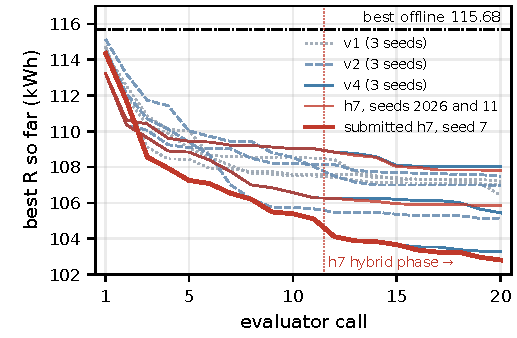
\includegraphics[width=\columnwidth]{figures/convergence.pdf}
\caption{每次调用后的平均最佳实测 $R$；阴影：种子间的范围。所有数值均为仿真器实测值。}
\label{fig:convergence}
\end{figure}

\textbf{RQ1：分块结构是否有效？} 去掉分块结构及两条依赖它的规则、其余不变，平均最终 $R$ 从 106.19 升到 107.84（$+1.65$~kWh，
$p=0.078$，各六个种子），并且平均而言 v4j 从第二次调用起就落后于 v4（第 10 次调用后的均值：108.48 对 107.12；
图~\ref{fig:convergence}）。单看这一差异，它没有达到 5\,\% 的显著性水平。v2 同样没有平台过滤和坐标重新施加，因此它把分块和
这两条规则分开了，但没有和后验份额、不重复规则以及第 1 次调用的八个跳跃点（从未命中）分开；v2 同样优于 v4j（$-1.37$~kWh，$p=0.041$）。在各分块下降变体之间，偏移偏置和分配都没有
可测地改变最终 $R$（两两比较 $p\ge0.48$），因此我们也把全部 15 次分块下降运行合起来与 v4j 比较：v4j 高 $+1.40$~kWh，$p=0.024$。
这两个比较都是在主比较之后选定的，所以我们把它们视为佐证，而不是证明。在这 15 次运行内部
可以看到这一机制。仅组合这一步（即每个新基点在尝试任何新移动之前相对上一个最好点的增益）就贡献了总下降的 33.0\,\%。组合点
有 83.7\,\% 低于当前最好点，加性预测~\eqref{eq:add} 的误差中位数为 $0.000$、平均绝对误差为 0.17~kWh（59\,\% 在 0.1 以内）；而
代理模型挑选的点平均比预测高 3.54~kWh（平均绝对误差 4.89），命中率为 4.2\,\%。在 43\,\% 的调用中，有两栋或以上的建筑在同一
批次中改进，因此组合不只是可用，而且确实被用上了。去掉分块后，代理模型挑选的点偏差更大（平均绝对误差 7.08），因为联合
移动离数据更远。

\begin{figure}[t]
\centering
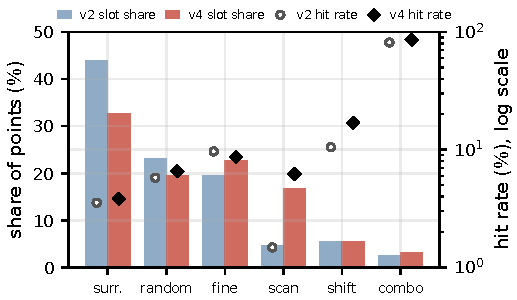
\includegraphics[width=\columnwidth]{figures/allocation.pdf}
\caption{各移动类别的点数份额（柱）与命中率（标记），汇总 v2 和 v4 的所有种子。命中指单块点低于其调用的基点，或基点与组合点（``combo''）低于上一个最好点。}
\label{fig:alloc}
\end{figure}

\textbf{RQ2：证据驱动的分配是否有效？} 没有可测的效果。在各六个种子上，v4 和 v2 分别停在 106.19 和 106.47（$-0.28$~kWh，
$p=0.76$）。平均而言 v4 在每一次调用都领先，但最多只领先 0.74~kWh（第 3 次调用），远在种子间的波动范围之内。这些规则确实做到了
设计要做的事（图~\ref{fig:alloc}）：后验份额把 11 个百分点的名额从代理模型挑选移走（44.0\,\% $\to$ 32.6\,\%；v4 中命中率为
3.8\,\%），转给扫描（4.6\,\% $\to$ 16.7\,\%）；扫描一旦跨出检测到的平台，命中率就从 1.5\,\% 升到 6.2\,\%。然而多出来的命中都很小：
扫描只贡献了 v4 下降量的 7.0\,\%，后期（第 11--20 次调用）从不同的权重向量返回本次运行已测过的 $R$ 的点所占比例仍在 31\,\% 左右（v2 为 32.6\,\%，
v4 为 31.3\,\%）。最初三个种子曾显示 0.93~kWh 的增益，另外三个种子使它消失了。

\textbf{其他变体与提交的策略。} 两次避免过早给每栋建筑锁定一种主导目标组合的尝试（顶点探测和并行通道），以及一个超参数
固定的代理模型，都没有超过 v4（三个种子上的均值分别为 106.26、106.86 和 106.22，v4 为 106.19）。一个独立的整批贝叶斯优化（加性 GP，每次
调用 24,000 个候选）在其唯一一次运行中达到 105.99，与 v4 的均值持平。提交的 h7 用提交的种子达到 102.81；它在自己的三个种子上的
第 1--11 次调用都与 v4 完全相同，因此在这三个种子上可以与 v4 配对，配对平均差为 $-0.09$（$-0.47$、$-0.24$、$+0.43$），即与 v4 无法区分。

\textbf{可复现性。} 从日志重新计算提交的运行，全部 20 个批次完全一致（最大 $|\Delta W|=0$）。在第二台机器上用评分运行包
跑另外两个种子，重放了第 1--11 次调用这 1,100 个点（2 个种子 $\times$ 11 次调用 $\times$ 50 个点）的 $R$：与对应的 v4 预演（用另一套框架、在另一台机器上运行）完全相同（只有
四个权重向量的最后一位不同，以及两个平局的候选交换了位置）。


\section{讨论与结论}
\label{sec:discussion}
分块下降在预测最弱的地方用实测替代了预测。它无需模型就能评估一个组合，因为加性（首次调用前已在训练行上检验）把实测的
单块效果变成了几乎精确的预报。分配规则显示了同一思路的边界：按实测命中率，名额如设计那样转向了扫描，但换来的命中太小，
在 20 次调用内改变不了最终 $R$。该方法不依赖于这个仿真器，而依赖两条性质：输入可以分成相互作用较弱的块，且每轮评估是
一个批次。

\textbf{局限。} (i) 种子的影响压过变体：v4 的六个种子相差 4.8~kWh，因此每个变体六个种子只能分辨较大的差异，分块消融正处在
显著性边缘（$p=0.078$），提交种子的 102.81 也不应被当作预期成绩（v4 平均 106.19）。一个独立的加性 GP 整批优化在其唯一一次
运行中与 v4 的均值持平，因此我们的结论是分块结构对这个策略有效，而不是分块下降优于调好的贝叶斯优化器。(ii) 所有比较都只用了
一个仿真器和一个问题；变体和种子是在本地运行上选定的，助教确认这是允许的，但提交的代码不含任何本地测得的点、数值或权重。
(iii) 评分结果取决于课程电脑能否发出相同的批次；运行包会检查 BLAS 配置，但无法强制保证。

\textbf{结论。} 在 1,000 个点的预算下，该策略在 v4 的不同种子上把 $R$ 从最佳训练行（115.76）降到 103.3--108.0，而我们最好的
离线提交为 115.68，课程基线为 119.09。可以推广的设计原则是：让批次中的每个点都成为结果可归因于单个块、并能在之后的组合
中复用的实验。

\bibliographystyle{IEEEtran}
\begin{thebibliography}{9}
\bibitem{rasmussen} C.~E. Rasmussen and C.~K.~I. Williams, \emph{Gaussian Processes for Machine Learning}. MIT Press, 2006.
\bibitem{turbo} D.~Eriksson, M.~Pearce, J.~Gardner, R.~D. Turner, and M.~Poloczek, ``Scalable global optimization via local Bayesian optimization,'' in \emph{NeurIPS}, 2019.
\bibitem{addgp} K.~Kandasamy, J.~Schneider, and B.~P{\'o}czos, ``High dimensional Bayesian optimisation and bandits via additive models,'' in \emph{ICML}, 2015.
\bibitem{bcd} S.~J. Wright, ``Coordinate descent algorithms,'' \emph{Mathematical Programming}, vol.~151, no.~1, pp.~3--34, 2015.
\end{thebibliography}
\end{document}
